\documentclass{article}

\usepackage{amsthm}
\usepackage{amsfonts}

\usepackage{amsmath}
\usepackage{amssymb}
\usepackage{fullpage}
\usepackage[utf8]{inputenc}
\usepackage{graphicx}
\usepackage[linguistics]{forest}
\usepackage[usenames]{color}
\usepackage{hyperref}
  \hypersetup{
    colorlinks = true,
    urlcolor = blue,       % color of external links using \href
    linkcolor= blue,       % color of internal links 
    citecolor= blue,       % color of links to bibliography
    filecolor= blue,        % color of file links
    }
    
\usepackage{listings}

\definecolor{dkgreen}{rgb}{0,0.6,0}
\definecolor{gray}{rgb}{0.5,0.5,0.5}
\definecolor{mauve}{rgb}{0.58,0,0.82}

\lstset{frame=tb,
  language=haskell,
  aboveskip=3mm,
  belowskip=3mm,
  showstringspaces=false,
  columns=flexible,
  basicstyle={\small\ttfamily},
  numbers=none,
  numberstyle=\tiny\color{gray},
  keywordstyle=\color{blue},
  commentstyle=\color{dkgreen},
  stringstyle=\color{mauve},
  breaklines=true,
  breakatwhitespace=true,
  tabsize=3
}

\theoremstyle{theorem} 
   \newtheorem{theorem}{Theorem}[section]
   \newtheorem{corollary}[theorem]{Corollary}
   \newtheorem{lemma}[theorem]{Lemma}
   \newtheorem{proposition}[theorem]{Proposition}
\theoremstyle{definition}
   \newtheorem{definition}[theorem]{Definition}
   \newtheorem{example}[theorem]{Example}
\theoremstyle{remark}    
  \newtheorem{remark}[theorem]{Remark}


\title{CPSC-354 Report}
\author{Darren Pak  \\ Chapman University}

\date{\today}

\begin{document}

\maketitle

\begin{abstract}
This is a culmination of all assignments and reports for CPSC-354 taught by Alex Kurz at Chapman University Fall 2022. 
\end{abstract}

\tableofcontents

\section{Introduction}\label{intro}

My name is Darren Pak and I am a computer science major at Chapman University with a minor in Data Analytics. My current goals as of Fall 2022 are to find interesting job opportunities and career paths that I find enjoyable and are able to sustain my lifestyle. 

\section{Homework}\label{homework}

This section contains solutions to homework assignments. 

\subsection{Week 1}

In Week 1, I will go over Euclid's Algorithm for Greatest Common Divisor and how it is implemented in C++.

\subsubsection{Euclid's Algorithm}

Euclid's Algorithm is defined as follows:

\medskip\noindent 
gcd(a,b):

\medskip\noindent 
Input: Two whole numbers (integers) called a and b, both greater than 0.

\medskip\noindent 
(1) if $$a > b$$ then replace a by a-b and go to (1).

\medskip\noindent 
(2) if $$b > a$$ then replace b by b-a and go to (1).

\medskip\noindent 
Output: a

\medskip\noindent
As described in \href{https://hackmd.io/@alexhkurz/SkqMtH0sK}{Alex Kurz Homework (Week 1)}

\subsubsection{Implementation in C++}

Below is the example for implementation of Euclid's Algorithm in C++:
\begin{lstlisting}
#include <iostream>

using namespace std;

int gcd(int a, int b) {
    while ((a != 1) && (b != 1)) {
        if (a > b) {
            a = a-b;
        }
        if (b > a) {
            b = b-a;
        }
        if (a == b) {
            return a;
        }
    }
    return a;
}

int main()
{
    cout<<gcd(9,33)<<endl;

    return 0;
}
\end{lstlisting}
In the function gcd, there is a while loop checking if either of the inputs are 1. This will eliminate cases where the GCD is already the lowest possible and as described in Euclid's algorithm, will return 1. Within the while loop, we go over the two rules in Euclid's Algorithm. The first being if a is greater than b then a is assigned to a - b. The second rule being if b is greater than a then b is assigned to b - a. Next we resolve the output and return a as the result.
\subsection{Week 2}
Week 2 is focused on recursion and functions in Haskell. For this assignment, I created 6 different functions using recursion in Haskell. Find the full \href{https://github.com/dapak2002/Pak-D-CPSC-354-Report/blob/main/src/hw2.hs}{Github Repository} here.

\subsubsection{Function Select Evens}
Here is a code snippet from the above mentioned Github Repository of the Select Evens function.
\begin{lstlisting}
select_evens :: [a] -> [a]
select_evens [] = []
select_evens (x:xs)
    |mod (length xs) 2 == 1 = x : select_evens xs
    |otherwise = select_evens xs
\end{lstlisting}
This function takes a list as an input and returns a list of only the even index elements. For example, from a list of ["a","b","c","d"] the function would return ["b","d"]. The first line of this function determines the input and outputs which are both lists of elements. The second line determines that an empty list from the function returns an empty list. This will become our indicator for ending recursion. Next we have an if statement saying that after the head, if there are an odd number of elements remaining, then the head element is of an even index. This means it would be appended to the returning list. If there is an even number of elements remaining, this means that the head element is of an odd index, meaning that the head element is skipped and will not be appended to the list. After all of the calculations have completed, the elements are appended to an empty list and added to the front in the order they were calculated.

Collaborated with Adrian Edralin for Week 2 Assignment.

\subsection{Week 3}
Week 3 assignment is focused around the Towers of Hanoi solving algorithm and how to evaluate functions. This game functions with n number of rings and 3 poles where the objective is to move all of the rings from the first pole (0) to the last pole (2). However, you are not able to stack larger rings on top of smaller rings while only moving 1 ring at a time. This game can be played at \href{https://www.mathsisfun.com/games/towerofhanoi.html}{mathisfun.com} in a simulated environment with different numbers rings.

\subsubsection{Rules of the Algorithm}
Our algorithm follows the following rules to solve this puzzle as described in \href{https://hackmd.io/@alexhkurz/rJQwvpyMY}{Towers of Hanoi (Week 3)}:
\begin{lstlisting}
hanoi 1 x y = move x y

hanoi (n+1) x y = 
	hanoi n x (other x y) 
	move x y 
	hanoi n (other x y) y
\end{lstlisting}

When expanded for n = 5 (5 rings), this becomes:
\begin{lstlisting}
hanoi 5 0 2  
	hanoi 4 0 1 
		hanoi 3 0 2
			hanoi 2 0 1 
				hanoi 1 0 2 = move 0 2 
				move  0 1
				hanoi 1 2 1 = move 2 1 
			move 0 2  
			hanoi 2 1 2  
				hanoi 1 1 0 = move 1 0  
				move  1 2  
				hanoi 1 0 2 = move 0 2
        move 0 1
        hanoi 3 2 1
            hanoi 2 2 0
                hanoi 1 2 1 = move 2 1
                move 2 0
                hanoi 1 1 0 = move 1 0
            move 2 1
            hanoi 2 0 1
                hanoi 1 0 2 = move 0 2
                move 0 1
                hanoi 1 2 1 = move 2 1
    move 0 2
    hanoi 4 1 2
        hanoi 3 1 0
            hanoi 2 1 2
                hanoi 1 1 0 = move 1 0
                move 1 2
                hanoi 1 0 2 = move 0 2
            move 1 0
            hanoi 2 2 0
                hanoi 1 2 1 = move 2 1
                move 2 0
                hanoi 1 1 0 = move 1 0
        move 1 2
        hanoi 3 0 2
            hanoi 2 0 1
                hanoi 1 0 2 = move 0 2
                move 0 1
                hanoi 1 2 1 = move 2 1
            move 0 2
            hanoi 2 1 2
                hanoi 1 1 0 = move 1 0
                move 1 2
                hanoi 1 0 2 = move 0 2
\end{lstlisting}
 This eventually gets simplified to the following moves where $$x->y$$ defines x being a ring moving from tower x to tower y:
 \begin{lstlisting}
 0->2
0->1
2->1
0->2
1->0
1->2
0->2
0->1
2->1
2->0
1->0
2->1
0->2
0->1
2->1
0->2
1->0
1->2
0->2
1->0
2->1
2->0
1->0
1->2
0->2
0->1
2->1
0->2
1->0
1->2
0->2
 \end{lstlisting}

\subsubsection{Analysis Questions}
In our original algorithm, it is shown that "hanoi" shows up 31 times. This is as the number of moves it takes to solve the puzzle meaning that the "hanoi" shows up the same number of times as the number of moves. 

\noindent For 1 ring, this is simple and would only take 1 move to solve. For 2 rings, this is 3 moves to solve. For 3 rings it is 7 moves to solve, for 4 rings it is 15 moves, and for 5 rings it is 31 moves. In this we see a pattern where for each additional ring, you double the amount of moves and add 1. In conclusion if n is the number of rings, this leads us to the equation of moves(n) = 2 * moves(n - 1) + 1, where moves(1) = 1 and n is greater than 0.

\subsection{Week 4}
This week is focused on concrete and abstract syntax trees which are essentially ways to parse equations. 
\subsubsection{Concrete Syntax Trees}

For the concrete syntax trees, we follow the rules and instructions as listed in the \href{https://hackmd.io/@alexhkurz/BkSgRX1GF}{Week 4 Report Instructions}. The rules are listed as following:
\begin{lstlisting}
Exp -> Exp '+' Exp1 
Exp1 -> Exp1 '*' Exp2              
Exp2 -> Integer            
Exp2 -> '(' Exp ')'  
Exp -> Exp1             
Exp1 -> Exp2 
\end{lstlisting}

\noindent 2+1:
\begin{forest}
  for tree={
    parent anchor=south,
    child anchor=north,
    fit=band,
  }
  [Exp
    [Exp
        [Exp1
            [Exp2
                [2]
            ]
        ]
    ]
    [+]
    [Exp1
        [Exp2
            [1]
        ]
    ]
  ]
\end{forest}

\noindent 1+2*3:
\begin{forest}
  for tree={
    parent anchor=south,
    child anchor=north,
    fit=band,
  }
  [Exp
    [Exp
        [Exp1
            [Exp2
                [1]
            ]
        ]
    ]
    [+]
    [Exp1
        [Exp1
            [Exp2
                [2]
            ]
        ]
        [*]
        [Exp2
            [3]
        ]
    ]
]
\end{forest}

\noindent 1+(2*3):
\begin{forest}
  for tree={
    parent anchor=south,
    child anchor=north,
    fit=band,
  }
[Exp
    [Exp
        [Exp1
            [1]
        ]
    ]
    [+]
    [Exp1
        [Exp2
        [(]
            [Exp
                [Exp1
                        [Exp1
                            [Exp2
                            [2]
                            ]
                        ]
                        [*]
                        [Exp2
                            [3]
                        ]
                ]
            ]
        [)]
        ]
    ]
]
\end{forest}

\noindent (1+2)*3:

\begin{forest}
for tree={
    parent anchor=south,
    child anchor=north,
    fit=band,
  }
  [Exp1
    [Exp1
        [Exp2
            [(]
            [Exp
                [Exp
                    [Exp1
                        [Exp2
                            [1]
                        ]
                    ]
                ]
                [+]
                [Exp1
                    [Exp2
                        [2]
                    ]
                ]
            ]
            [)]
        ]
    ]
    [*]
    [Exp2
        [3]
    ]
]
\end{forest}

\noindent 1+2*3+4*5+6:
\begin{forest}
    for tree={
    parent anchor=south,
    child anchor=north,
    fit=band,
  }
[Exp
    [Exp
        [Exp
            [Exp
                [Exp1
                    [Exp2
                        [1]
                    ]
                ]
            ]
            [+]
            [Exp1
                [Exp1
                    [Exp2
                        [2]
                    ]
                ]
                [*]
                [Exp2
                    [3]
                ]
            ]
        ]
        [+]
        [Exp1
            [Exp1
                [Exp2
                    [4]
                ]
            ]
            [*]
            [Exp2
                [5]
            ]
        ]
    ]
    [+]
    [Exp1
        [Exp2
            [6]
        ]
    ]
]
\end{forest}

\subsubsection{Abstract Syntax Trees}
For the abstract syntax trees, we can find a similar instructions here at \href{https://hackmd.io/@alexhkurz/BkqOWbgMF}{Week 4 Report for Abstract Syntax Trees}. The rules again are listed as following:
\begin{lstlisting}
Plus.   Exp ::= Exp "+" Exp1 ;
Times.  Exp1 ::= Exp1 "*" Exp2 ;
Num.    Exp2 ::= Integer ;

coercions Exp 2 ;
\end{lstlisting}
2+1:
\begin{forest}
    for tree={
    parent anchor=south,
    child anchor=north,
    fit=band,
  }
  [Plus
    [Num
        [2]
    ]
    [Num
        [1]
    ]
]
\end{forest}

\noindent 1+2*3:
\begin{forest}
    for tree={
    parent anchor=south,
    child anchor=north,
    fit=band,
  }
  [Plus
    [Num
        [1]
    ]
    [Times
        [Num
            [2]
        ]
        [Num
            [3]
        ]
    ]
]
\end{forest}

\noindent 1+(2*3):
\begin{forest}
    for tree={
    parent anchor=south,
    child anchor=north,
    fit=band,
  }
  [Plus
    [Num
        [1]
    ]
    [Times
        [Num
            [2]
        ]
        [Num
            [3]
        ]
    ]
]
\end{forest}

\noindent (1+2)*3
\begin{forest}
for tree={
    parent anchor=south,
    child anchor=north,
    fit=band,
  }
[Times
    [Plus
        [Num
            [1]
        ]
        [Num
            [2]
        ]
    ]
    [Num
        [3]
    ]
]
\end{forest}

\noindent 1+2*3+4*5+6:
\begin{forest}
for tree={
    parent anchor=south,
    child anchor=north,
    fit=band,
  }
[Plus
    [Plus
        [Plus
            [Num
                [1]
            ]
            [Times
                [Num
                    [2]
                ]
                [Num
                    [3]
                ]
            ]
        ]
        [Times
            [Num
                [4]
            ]
            [Num
                [5]
            ]
        ]
    ]
    [Num
        [6]
    ]
]
\end{forest}

\noindent In regards to the abstract syntax tree of 1+2+3, this would be identical to (1+2)+3 because we read operations from left to right which matches this order of parentheses.

\subsection{Week 5}
Here are the evaluations found in \href{https://hackmd.io/@alexhkurz/S1D0yP8Bw}{Homework 5}.
\begin{lstlisting}
"x":
Prog (EVar (Id "x"))

"x x":
Prog (EApp (EVar (Id "x")) (EVar (Id "x")))

"x y":
Prog (EApp (EVar (Id "x")) (EVar (Id "y")))

"x y z":
Prog (EApp (EApp (EVar (Id "x")) (EVar (Id "y"))) (EVar (Id "z")))

"\ x.x":
Prog (EAbs (Id "x") (EVar (Id "x")))

"\ x.x x":
Prog (EAbs (Id "x") (EApp (EVar (Id "x")) (EVar (Id "x"))))

"(\ x . (\ y . x y)) (\ x.x) z":
Prog (EApp (EApp (EAbs (Id "x") (EAbs (Id "y") (EApp (EVar (Id "x")) (EVar (Id "y"))))) (EAbs (Id "x") (EVar (Id "x")))) (EVar (Id "z")))

"(\ x . \ y . x y z) a b c":
Prog (EApp (EApp (EApp (EAbs (Id "x") (EAbs (Id "y") (EApp (EApp (EVar (Id "x")) (EVar (Id "y"))) (EVar (Id "z"))))) (EVar (Id "a"))) (EVar (Id "b"))) (EVar (Id "c")))
\end{lstlisting}

\noindent The 2-D abstract syntax trees are found at \href{https://github.com/dapak2002/Pak-D-CPSC-354-Report/blob/main/src/HW5.pdf}{the Github pdf here}.

\noindent The abstract syntax trees for \href{https://hackmd.io/@alexhkurz/H1e4Nv8Bv}{Homework 5 part 2} can be found at the pdf of the evaluations in \href{https://github.com/dapak2002/Pak-D-CPSC-354-Report/blob/main/src/Hw5-pt2.pdf}{the Github file}.

\subsection{Week 6}
This week is focused on evaluating expressions using Lambda Calculus. An example of this can be found in \href{https://youtu.be/for3Meg1Lbc}{Dr. Kurz's tutorial}. 

\subsubsection{Expression Evaluation}
The expression we will be taking a look at this week is:
\begin{lstlisting}
(\exp . \two . \three . exp two three)
(\m.\n. m n)
(\f.\x. f (f x))
(\f.\x. f (f (f x)))
\end{lstlisting}
Using the method described in the tutorial above, this evalutates to:
\begin{lstlisting}
(\exp . \two . \three . exp two three)
(\m.\n. m n)
(\f.\x. f (f x))
(\f.\x. f (f (f x)))
=
(\two . \three . (\m.\n. m n) two three)
(\f.\x. f (f x))
(\f.\x. f (f (f x)))
=
(\three . (\m.\n. m n) (\f.\x. f (f x)) three)
(\f.\x. f (f (f x)))
= 
((\m.\n. m n) (\f.\x. f (f x)) (\f.\x. f (f (f x))))
=
((\m.\n. m n) (\f2.\x2. f2 (f2 x2)) (\f3.\x3. f3 (f3 (f3 x3))))
=
((\n. (\f2.\x2. f2 (f2 x2)) n) (\f3.\x3. f3 (f3 (f3 x3))))
=
(((\f2.\x2. f2 (f2 x2)) (\f3.\x3. f3 (f3 (f3 x3)))))
=
(((\x2. (\f3.\x3. f3 (f3 (f3 x3))) ((\f3.\x3. f3 (f3 (f3 x3))) x2))))
=
(((\x2. (\x3. ((\f3.\x3. f3 (f3 (f3 x3))) x2) (((\f3.\x3. f3 (f3 (f3 x3))) x2) (((\f3.\x3. f3 (f3 (f3 x3))) x2) x3))))))
=
(((\x2. (\x3. ((\x3. x2 (x2 (x2 x3)))) (((\f3.\x3. f3 (f3 (f3 x3))) x2) (((\f3.\x3. f3 (f3 (f3 x3))) x2) x3))))))
=
(((\x2. (\x3. ((\x3. x2 (x2 (x2 x3)))) (((\x3.  x2 ( x2 ( x2 x3)))) (((\f3.\x3. f3 (f3 (f3 x3))) x2) x3))))))
=
(((\x2. (\x3. ((\x3. x2 (x2 (x2 x3)))) (((\x3.  x2 ( x2 ( x2 x3)))) (((\x3.  x2 ( x2 ( x2 x3)))) x3))))))
=]
(\x2. (\x3. (\x3. x2 (x2 (x2 x3))) ((\x3.  x2 ( x2 ( x2 x3))) (((\x3.  x2 ( x2 ( x2 x3)))) x3))))
=
(\x2. ((\x3. x2 (x2 (x2 ((\x3. x2(x2(x2 x3))) (((\x3.  x2 ( x2 ( x2 x3)))) x3)))))))
=
(\x2. (\x3. x2 (x2 (x2 ((x2 ( x2 ( x2 (((\x3.  x2 ( x2 ( x2 x3)))) x3)))) )))))
=
(\x2. (\x3. x2 (x2 (x2 (x2 ( x2 ( x2 ((x2 ( x2 (x2 x3)))))))))))
=
\x2. (\x3. x2(x2(x2(x2(x2(x2(x2(x2(x2 x3)))))))))
\end{lstlisting}
In the first line, the function is defined as 'exp' with two terms. By analyzing the evaluation we find that the function is essentially the first term to the exponent of the second term.

\subsection{Week 7}
\subsubsection{Lambda Calculus and Variable Interpretation}
This week is understanding bound and free variables. A bound variable is a variable in a function that can be replaced with any other new variable and still retain the same meaning. A free variable is NOT a bound variable as it can some variables can only be used in certain context. My understanding of this terminology is that free variables must have a certain meaning in the context of the application and therefore cannot be replaced, whereas bound variables can be filled in and replaced as seen fit in the application. To look at some examples, we can take the \href{https://github.com/alexhkurz/programming-languages-2022/blob/main/src/LambdaNat0/src/Interpreter-fragment.hs}{Interpreter-fragment.hs} from Alex Kurz as example in the context of lambda calculus.
\begin{lstlisting}

# The heart of the interpreter ... all else is "boilerplate"

-- evaluate using the strategy call-by-name
evalCBN :: Exp -> Exp  
evalCBN (EApp e1 e2) = case (evalCBN e1) of
    (EAbs i e3) -> evalCBN (subst i e2 e3)
    e3 -> EApp e3 e2
evalCBN x = x 

-- generate a fresh name
fresh :: Exp -> String

-- subst id s e performs capture avoiding substitution of id by s in e
subst :: Id -> Exp -> Exp -> Exp
subst id s (EVar id1) | id == id1 = s
                      | otherwise = EVar id1
subst id s (EApp e1 e2) = EApp (subst id s e1) (subst id s e2)
subst id s (EAbs id1 e1) = 
    -- to avoid variable capture, we first substitute id1 with a fresh name inside the body of the lambda-abstraction, obtaining e2. Only then do we proceed to apply substitution of the original s for id in the body e2.
    let f = fresh (EAbs id1 e1)
        e2 = subst id1 (EVar f) e1 in 
        EAbs f (subst id s e2)
\end{lstlisting}

From this we see that in lines 5-7 there are 4 different variables, (i, e1, e2, and e3). In the context of lambda calculus, i is a free variable because this is used to represent lambda. Therefore it cannot be replaced by a different value and must be lambda in this use case. e1, e2, and e3 are bound variables because depending on the expression these will be replaced by other variables without changing the meaning of the expression. The binders for e1, e2, and e3 are represented in the functions of the interpreter. These are EApps, EAbs, subst, and evalCBN. The scope is only to the function and is limited to only evalCBN.

\medskip
If we look at lines 18-22 we see the same patterns. In this case id is representing lambda and is a free variable because it cannot be replaced in this context without changing the meaning. The other variables s, e1,e2, and f are all bound variables because they can be replaced without changing the meaning of the expression. In this case the binders for s, e1, e2, and f are the same functions described in the interpreter being EApps, EAbs, and subst. The scope is limited only to the fucntion defined as subst.

\subsubsection{evalCBN Haskell interpreter}
\medskip
Looking at the function evaLCBN in \href{https://github.com/alexhkurz/programming-languages-2022/blob/main/src/LambdaNat0/src/Interpreter-fragment.hs}{Interpreter-fragment.hs} we use this to evaluate two different functions.
\begin{lstlisting}
(\x.x)((\y.y)a)
evalCBN ((EApp (EAbs (Id "x") (EVar (Id "x"))) (EApp (EAbs (Id "y") (EVar (Id "y"))) (EVar (Id "a"))))) = -- line 6
evalCBN (subst (Id "x") (EApp (EAbs (Id "y") (EVar (Id "y"))) (EVar (Id "a"))) (Evar (Id "x"))) = = -- line 15
evalCBN (EApp (EAbs (Id "y") (EVar (Id "y"))) (EVar (Id "a"))) = -- line 6
evalCBN (subst (Id "y") (EVar (Id "a")) (EVar (Id "y"))) = -- line 15
evalCBN (EVar (Id "a")) = -- line 8
EVar (Id "a")

(\x.\y.x) y z
evalCBN (EApp (EAbs (Id "x") (EAbs (Id "y") (EVar (Id "x")))) (EVar (Id "y")) (EVar (Id "z"))) = -- line 6
evalCBN(subst (Id "x") (EAbs (Id "y") (EVar (Id "x"))) (EVar (Id "y")) (EVar (Id "z"))) = -- line 15
evalCBN(EApp (EAbs (Id "y") (EVar (Id "y"))) (EVar (Id "z"))) = -- line 6
evalCBN (subst (Id "y") (EVar (Id "z")) (EVar (Id "y"))) = -- line 15
evalCBN (EVar (Id "z")) = -- line 8
EVar (Id "z")
\end{lstlisting}
\subsubsection{ARS Mapping}
The ARS maps as specified in \href{https://hackmd.io/@alexhkurz/BJ7AoGcVK}{Week 7 HW} can be found at the  \href{https://github.com/dapak2002/Pak-D-CPSC-354-Report/blob/main/src/ARSmaps.pdf}{ARSmaps.pdf} on GitHub. 

\subsection{Week 8}
This week we look at rewriting rules and how they can be terminating and go more into depth about normal forms. First we look at the assignment as described in \href{https://hackmd.io/@alexhkurz/Syn23oMHF}{String Rewriting Exercise}.

\subsubsection{String Rewriting}
From the previously mentioned exercise page, the first set of rules will be as follows:
\begin{lstlisting}
  aa -> a
  bb -> b
  ba -> ab
  ab -> ba
\end{lstlisting}
We follow-up by asking these questions:

\medskip
Why does the ARS not terminate?
What are the normal forms?

\medskip
The ARS does not terminate because line 3 (ba to ab) and line 4 (ab to ba) can cause a loop. Since it is essentially commutative that ab can go to ba and back, there is no definitive ending to "ab" and "ba".

\medskip
Can you change the rules so that the new ARS has unique normal forms (but still has the same equivalence relation)?

\medskip
Yes you can change the rules so that the new ARS has UNF and maintain the same equivalence relation. An example of this can be the rules:
\begin{lstlisting}
  ab -> c
  ba -> c
\end{lstlisting}

\medskip
What do the normal forms mean? Describe the function implemented by the ARS.

\medskip
A normal form essentially means a value or expression that cannot be simplified further by any rules. This function is removing all duplicate values and allowing one to alternate the expression from "ab" to "ba" freely. 

\section{Week 9} This week, the lessons are focused towards understanding more about ARS and we will perform an analysis on a set of rules. I will first talk about some milestones set for the project to put steps that are measurable towards progress of completion.

\subsubsection{Final Project Milestones}
For the final project, here are the due dates and requirements for each:

\medskip
By November 6th: Find of the top 10 most used programming languages in the last year. This will be based on the site, \href{https://madnight.github.io/githut/#/pull_requests/2021/4}{Githut 2.0} which is a site that rates different languages based on their "popularity" metric.

\noindent
Requirements: A list of the top 10 most used programming languages and a written report on reasons to include each one.

\medskip
By November 13th: Find at least a couple sentiment analysis program for Reddit and write a list of interesting features that may come along with each one. This includes pro's and con's of each program and also the ease of use to get each one working.

\noindent
Requirements: A report that includes: a list of possible NLP sentiment analysis programs for Reddit, a list of Reddit pages (may not be the default page for the language) 

\medskip
By November 20th: Create the report prototype for each programming language on Reddit. This means using a sentiment analysis program to find a list of the most commonly used words mentioned on the Reddit page within the last year. From this I can determine whether or not the program we chose is correct and any changes I may need to make in the procedure. This prototype will include a report on reasons why each word is most likely mentioned and any interesting points about the topics.

\medskip
By December 6th: Finalize the method in which sentiment analysis will be done. This is to create a list of steps or a report on how to create each model so steps may be repeated in the future. Also this is included for reference on how steps may be improved later on.

\noindent
Requirements: A procedure guide with step-by-step instructions on how to complete the sentiment analysis and find the list of the top 10 words.

\medskip
By the final due date: Complete a report on the top 10 most used programming languages and how sentiment analysis was used to find the top 10 most commonly used words on their Reddit. From this, analyze any patterns and give a report on the history of the language and what it was originally intended for. Show a comparison to how this has evolved into the use case today and what kind of discussion surrounds the language on forums from users.

\subsubsection{ARS Analysis}
The rules given to use are described as follows:
\begin{lstlisting}
ba -> ab
ab -> ba
ac -> ca
ca -> ac
bc -> cb
cb -> bc
 
aa -> b
ab -> c
ac ->  
bb ->
cb -> a
cc -> b
\end{lstlisting}

From this we ask ourselves a few questions:

\medskip
What are the normal forms and how can we be sure we have found every normal form?

\noindent From the rules we can understand that the first 6 lines only transpose between two forms, and the next 6 rules are how we determine normal forms. From this, we see that "a", "b", "c", and {} are the normal forms. This is because for the combinations (ab, ac, ba, bc, ca, cb) we have a rule to alternate to a reversed form (ab to ba). This is a result of every combination having a way to end in a single value (by the last 6 rules) which results to the normal forms.

\medskip
Is the ARS terminating?

\noindent
No this ARS is not terminating because there are many ways to infinitely loop. The transpose rules (ex. rule 1 and 2) are all culprits to this and can cause an infinitely loop if you decide to go between ab and ba an infinite amount of times.

\medskip
Are there unique normal forms?

\noindent
No the normal forms are not unique. Again, the transpose rules mean that there are no unique normal forms. From the same example, "ab" and "ba" both result to "c" which means the normal forms are not unique.

\medskip
Now replace in your mind the one-step rewrite relation -> by an equality =. Given this notion of =, are all the normal forms different?

\noindent
All normal forms are not different. Because we have rules to transpose from a reversed form, this means not all of the normal forms are different. For example, "ab" and "ba" both result to "c" and when we write an equality relation, although the results of "c" = "c", "ab" and "ba" are not equal.

\subsection{Week 10}
In week 10 we continue lambda calculus reductions and computations. For this week's exercise the problem to solve is defined in \href{https://hackmd.io/@alexhkurz/rJEeYqZtw}{Lambda Calculus: Extensions} by Alex Kurz. This problem is to be solved using previously attempted equational reasoning methods.

\subsubsection{Solving fix_F 2}
The problem is defined as follows:
\begin{lstlisting}
\f.\n if n == 0 then 1 else f(n-1)*n
fix_F \approx F fix_f
\end{lstlisting}

This is solved using equational reasoning as follows (image is also uploaded to \href{https://github.com/dapak2002/Pak-D-CPSC-354-Report/blob/main/src/HW10.png}{Github}):

\begin{figure}[htp]
    \centering
    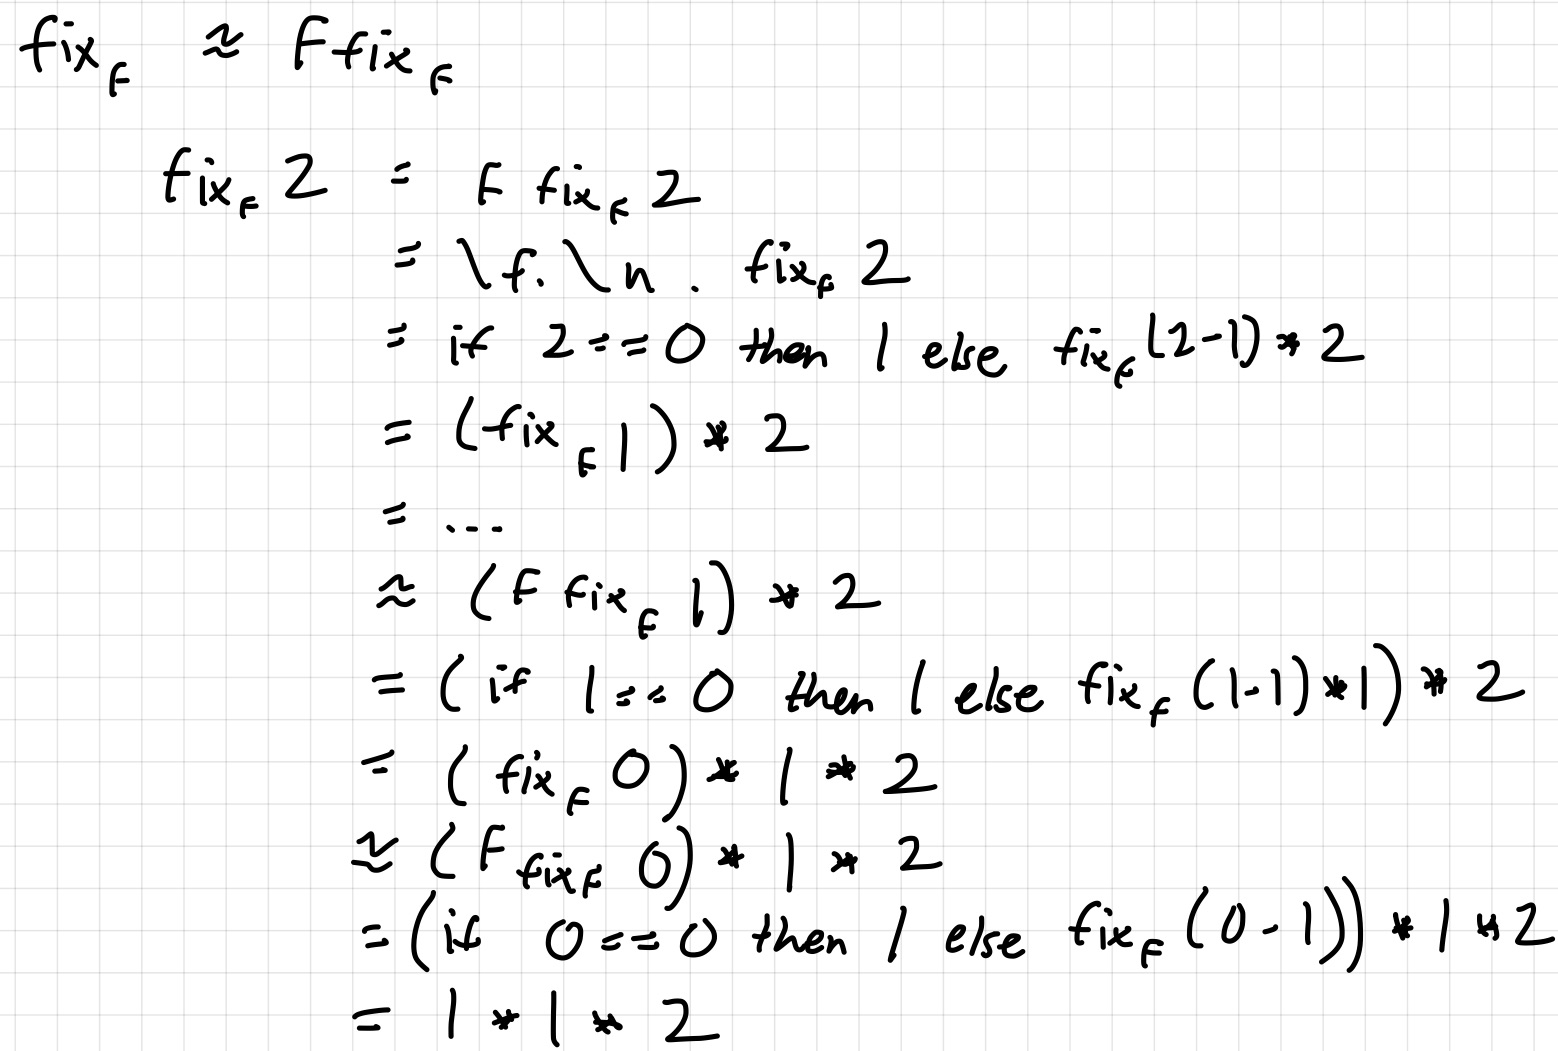
\includegraphics[width=14cm]{HW10.png}
\end{figure}

\subsection{Week 11}
For this week we analyze the article of \href{https://hackmd.io/@alexhkurz/rJ9O5tZSo}{composing contracts} as mentioned by Alex Kurz in this assignment. I then asked the following question in a discussion and replied to a few of my peers questions.

\subsubsection{My Question}
For my question, I want to focus on the section about combining contracts. What is interesting to me is that contracts can be combined, but there was no example of any type of tree that can be created through combining contracts. For example, if a contract would return some value A and from A we create another contract to return B, then another to return C this would look like A -> B -> C. This is of course assuming that all of the conditions from the contracts are being met and through combining contracts this is also combining the conditions.

Is there a transitive property that can be written to go A ->C? And if so what would the abstract syntax tree look like? This also asks another questions if there are other unexplored properties of contracts.

\subsubsection{Responses}
These are the responses to my peers.

\medskip
By Luke Boctor: Why did the creators decide to design and implement their contract valuation engine in Haskell? Could there be a better host language for their objectives?

\medskip
Answer: I believe that Haskell is chosen for this implementation because of the unique way that rules/substitution work in Haskell. In this case, contracts benefit from being able to write the equivalence relationships easily using Haskell's "=".  A contract with a condition can be resolved by simply evaluating which in Haskell is through the nature of the language to simplify the expression as much as possible using various rules. 

\medskip
By Devon Foy: Contracts aren't the only area of finance that could potentially benefit from the concepts in the paper. How could this technology be expanded on to compose and value combinations of other financial instruments such as mortgage backed securities?

\medskip
Another potential area of use could be the retail sector. It seems contracts are another way to create "trades" are ensure that a condition is fulfilled with a result at the end. For example, in a used item market where items are being sold, bought, and traded. The values of these items may not all be tracked properly and therefore contracts could be a solution to ensure all of the requirements and outputs get resolved.

\subsection{Week 12}
This week is focused on Hoarse Logic and finding invariants as well as resolving the pre/postconditions. 

\subsubsection{Condition Analysis}
The condition we will be analyzing is:
\begin{lstlisting}
while (x!=0) do z:=z*y;  x:= x-1 done
\end{lstlisting}

\medskip
To start off our analysis, we will be finding the precondition as well as the postcodition in order to get a better understanding of the problem. By looking at the equation, we can understand that x is greater than or equal to 0 because of "while (x!=0)" and we also understand that z must start at 1 so that "z=z*y" is not nullified by a 0, and therefore starts at 1 so that z is able to increase. From this, we find that the precondition would be: $$x \geq 0 \wedge z = 1$$ To find the post condition, we take a better understanding of the equation as x is the exponent of y with z being the result. In an equation this would look like: $$z = y^x$$

\subsubsection{Hoare Logic}
To find the Hoare Rule for the above while loop, we can rewrite the equation as:
$$\frac{\{I\}S\{I\}}{\{I\}while B do S done \{ \neg B \wedge I \}}$$

In this case, S represents: $$z := z * y; x:= x - 1$$ This means that I represents the while loop invariant. By doing an example of a given number, we can resolve a new invariant through using numbers. For example, if x is 10, y is 2, and z is 1, then we find that the result of this example using algebra will be $$z = 2^{(10-x)}$$ Using the precondition and postcondition as stated in the earlier section, we create $$z = y^{(t - x)}$$ where t represents the number of times the loop occurs. Replacing y with k, the invariant results to $$z = k^{(t - x)}$$

\section{Project}

\subsection{Introduction}

For my final project, I analyzed the top 10 most popular programming language subreddits to determine key characteristics and attributes of each language. Subreddits are communities on the social media platform “Reddit” that offer a forum for developers and users alike to discuss various topics. Each subreddit is focused on a specific topic, and in this case, we will take a look at the programming language subreddits to see if we can analyze discussions and find out more about the language. This project aims to provide insight into how each programming language is used, including common applications, errors and error messages, and tools and packages that are frequently used by developers.

\subsection{Specification}

\subsubsection{Prototype Specifications}
To find the top 10 most popular programming languages, I used the website \href{https://madnight.github.io/githut/#/pull_requests/2022/3}{GitHut 2.0}. This site tracks various Github statistics such as pull requests, pushes, stars, and issues. I based my decision off of the number of pull requests as this is the most reliable way to determine how many meaningful changes/versions were made. The main prototype of the project is a Python script that uses the `praw` module from Reddit. This package allows you to use Reddit API calls and access posts from each subreddit. Since the top posts are continuously changing, the time is output at the top of the file. The script defines a list of subreddit names to be processed. For each subreddit in the list, the script retrieves the subreddit, obtains the top 100 posts in the subreddit using the hot() method, and creates a frequency dictionary to store the frequency of each word in the subreddit. The script then iterates through the top posts, extracts the text of each post, splits the text into words, removes punctuation, and lowercases the words. It counts the frequency of each word and stores it in the frequency dictionary and then removes certain words from the frequency dictionary based on the manually added list of words to remove. After, it sorts the frequency dictionary in descending order by frequency and prints the top 10 words and their frequencies for the subreddit. Finally, the script writes the words and frequencies to a CSV file with the subreddit name as the file name.

\subsubsection{Report Specifications}
In the documentation, I will be going over each programming language. This means taking a look at what each of the words mean, why each of the words were included, interesting topics about the frequencies, and in the end going over the differences and summaries of each of the languages.

\subsection{Prototype}

\subsubsection{GitHut 2.0 Search}
From GitHut 2.0 on December 18th, 2022 at 1:28 PM, the following programming languages were at the top for pull requests from greatest to least:

\noindent
Python, Java, C++, Go, JavaScript, TypeScript, PHP, Ruby, C, and C#

\subsubsection{Reddit Python Prototype}
I chose to write the main prototype in Python as it is the easiest to follow along with, and has all of the functionality that I wanted. The version of Python I used is 3.9.15. This was run on an arm64-based Macbook with Python installed through Conda and uses pygplates. You will need to install are the \verb |praw| package and also need access to a Reddit developer account (which can applied for on the Reddit website). By creating a new application on Reddit, this gives you access to both the client ID and secret code which must be replaced in order to run the program. The prototype Python script can also be found here on \href{https://github.com/dapak2002/Programming-Language-Reddit-Scraper}{GitHub}:
\begin{lstlisting}
import praw
import string
import csv

# Replace YOUR_CLIENT_ID and YOUR_CLIENT_SECRET with your Reddit API key and secret
reddit = praw.Reddit(client_id="YOUR_CLIENT_ID", client_secret="YOUR_CLIENT_SECRET", user_agent="my_user_agent")

subreddit_names = ["python" , "java", "cpp", "golang" , "javascript" , "typescript", "golang" , "csharp" , "cpp" , "c_programming"]  # List of subreddit names to process
subreddit_names = ["java" , "typescript", "javascript", "php" , "ruby" , "python", "golang" , "csharp" , "cpp" , "c_programming"]  # List of subreddit names to process

for subreddit_name in subreddit_names:
    subreddit = reddit.subreddit(subreddit_name)  # Get the subreddit

    top_posts = subreddit.hot(limit=100)  # Get the top 100 posts in the subreddit

    frequency = {}  # Dictionary to store the frequency of each word

    for post in top_posts:
        # Get the text of the post
        text = post.title + " " + post.selftext

        # Split the text into words and remove punctuation
        words = text.split()
        words = [word.lower().translate(str.maketrans('', '', string.punctuation)) for word in words]

        # Count the frequency of each word
        for word in words:
            if len(word) >= 4:  # Only consider words with at least 4 characters
                if word in frequency:
                    frequency[word] += 1
                else:
                    frequency[word] = 1

    # Remove certain words from the frequency dictionary
    stop_words = [ "really" , "something" , "should" , "make" , "been" , "help" , "other" , "please" , "here" , "which" , "using" , "about" , "into" , "know" , "where" , "like", "when" , "only" , "also" , "used" , "there" , "golang" , "python" , "string" , "this", "have" , "with" , "your", "want", "that" , "need" , "just", "will" ,"from" , "some" , "within" , "does" , "would", "what" , "more" , "java" , "typescript", "javascript", "php" , "ruby" , "python", "golang" , "csharp" , "cpp" , "c_programming"]  # Add any other words you want to remove
    for word in stop_words:
        if word in frequency:
            del frequency[word]

    # Sort the frequency dictionary in descending order
    sorted_frequency = sorted(frequency.items(), key=lambda x: x[1], reverse=True)

    # Print the top 10 words with their frequency, preceded by the subreddit name
    print(f"Top words in /r/{subreddit_name}:")
    for i in range(10):
        word, frequency = sorted_frequency[i]
        print(f"{word}: {frequency}")
    print()  # Print an empty line to separate the output for different subreddits

    # Write the words and frequencies to a CSV file
    with open(f"{subreddit_name}.csv", "w", newline="") as csvfile:
        writer = csv.writer(csvfile)
        writer.writerow(["word", "frequency"])  # Write the header row
        for word, frequency in sorted_frequency:
            writer.writerow([word, frequency])
\end{lstlisting}

\medskip
As described above in the specifications, the script will search the subreddits listed in \verb |subreddit_names| and will find the top 100 posts. These fields are able to be edited for example, by changing the subreddits or looking at the top 1000 posts. Another feature is I have made the length of the word need to be at least 4 characters to be considered. This is to remove common conjunctions like "a", "an", and "to" automatically, so I don't have to add them to the remove words list. The remove words list is all of the words I found uninteresting. These needed to be removed in order to find our true objective of unique and interesting topics about each programming language. The code also outputs to a CSV file which I implemented for future releases of other programs that may find this kind of data useful. The time is output at the top to know when the posts were taken from.

\medskip
The information output from the code listed above on December 18th, 2022:
\begin{lstlisting}
Timestamp: 2022-12-18 15:03:43.182166
Top words in /r/python:
data: 33
project: 31
file: 31
time: 29
code: 26
people: 23
files: 22
framework: 20
create: 19
dash: 18

Top words in /r/java:
spring: 26
support: 23
class: 18
time: 16
code: 15
data: 15
value: 15
examples: 14
boot: 13
services: 13

Top words in /r/cpp:
code: 48
class: 39
coroutine: 30
library: 28
performance: 22
rocksdb: 22
such: 20
function: 20
time: 19
threads: 19

Top words in /r/golang:
func: 48
code: 43
type: 38
struct: 37
return: 35
error: 33
interface: 33
client: 32
server: 31
data: 26

Top words in /r/javascript:
code: 37
askjs: 16
react: 12
2022: 9
library: 8
website: 8
data: 8
programming: 7
vuejs: 6
source: 6

Top words in /r/typescript:
type: 167
const: 52
code: 48
error: 47
types: 42
function: 36
interface: 33
return: 29
number: 26
array: 22

Top words in /r/php:
class: 24
laravel: 22
code: 18
function: 16
framework: 15
project: 14
file: 13
docker: 13
version: 12
magic: 12

Top words in /r/ruby:
rails: 22
code: 14
method: 11
data: 9
looking: 8
array: 8
post: 7
install: 7
over: 6
hello: 6

Top words in /r/c_programming:
function: 65
struct: 59
program: 54
file: 54
return: 50
char: 48
code: 46
array: 46
include: 40
void: 29

Top words in /r/csharp:
public: 46
code: 45
data: 30
void: 19
class: 18
input: 15
private: 15
most: 14
application: 14
double: 14
\end{lstlisting}

\subsection{Documentation}
Each of the programming languages has been separated into sections with my analysis and summaries. The output is taken on December 18th, 2022.

\subsubsection{Python}
\begin{tabular}{ | l | r | p{7cm} | }
\hline
Word & Frequency & Meaning \\
\hline
data & 33 & refers to information that is stored or created \\
\hline
project & 31 & refers to a specific task or activity with a defined outcome \\
\hline
file & 31 & refers to a collection of data stored in a computer system \\
\hline
time & 29 & refers to the duration during which an event or set of events takes place \\
\hline
code & 26 & refers to a set of instructions or statements written in a programming language \\
\hline
people & 23 & refers to human beings in general or a group of individuals \\
\hline
files & 22 & plural of file, (files is a hot topic in Python) \\
\hline
framework & 20 & refers to a set of ideas or concepts that provide a structure for something \\
\hline
create & 19 & refers to the process of making or producing something \\
\hline
dash & 18 & this can either be the symbol "-" or the data visualization framework package \\
\hline
\end{tabular}

\medskip
Python is one of the easier programming languages because of all its functions and packages that come included. Most of the words here refer to traditional software development such as data, project, file, and code. The unique ones are people, time, framework, create and dash. People most likely is here because the discussions are about developers or users. Framework is included because Python can often be used as a structure for projects cause of its simplicity. Create is most likely here because again, Python's simplicity and ease of use to create anything. Dash is the framework package used for data visualization in Python and is a helpful tool. Many tools like Dash and Pandas make Python a favorite for data visualization.

\subsubsection{Java}
\begin{tabular}{ | l | r | p{7cm} | }
\hline
Word & Frequency & Meaning \\
\hline
spring & 26 & refers to a lightweight framework used to build Java applications \\
\hline
support & 23 & refers to assistance or help provided for a particular purpose \\
\hline
class & 18 & refers to a type of data structure used in object-oriented programming languages \\
\hline
time & 16 & refers to the duration during which an event or set of events takes place \\
\hline
code & 15 & refers to a set of instructions or statements written in a programming language \\
\hline
data & 15 & refers to information that is organized for analysis or interpretation \\
\hline
value & 15 & refers to the worth or importance of something \\
\hline
examples & 14 & refers to instances or demonstrations used to illustrate a concept or point \\
\hline
boot & 13 & refers to the process of starting a computer or device \\
\hline
services & 13 & refers to actions performed for the benefit of others, or a specific type of work or task \\
\hline
\end{tabular}

\medskip
Java is the first language I actually learned and is an interesting one because there are multiple Java subreddits such as r/java, r/javahelp, and r/learnjava. I chose the basic r/java because it included the most news and discussion about the programming language rather than the code. This removes typical keywords that get over used and overall I feel pretty good about the results. Here we see the top word being spring. Spring is a Java framework used to build Java applications. There is a lot of discussion around this because it is easy to use and helps simplify the software development process. Other discussions talk about support which redirect to r/javahelp. Again we see more software development terms like class, time, code, data, value, and boot. This subreddit focused a lot on discussions as seen in examples and services.

\subsubsection{C++}
\begin{tabular}{ | l | r | p{7cm} | }
\hline
Word & Frequency & Meaning \\
\hline
code & 48 & refers to a set of instructions or statements written in a programming language \\
\hline
class & 39 & refers to a type of data structure used in object-oriented programming languages \\
\hline
coroutine & 30 & refers to a function that can be paused and resumed, allowing for efficient use of resources in concurrent programming \\
\hline
library & 28 & refers to a collection of pre-compiled code that can be used in a program \\
\hline
performance & 22 & refers to the effectiveness or efficiency of a system or process \\
\hline
rocksdb & 22 & refers to an embedded database system focused on storage speeds \\
\hline
such & 20 & refers to a person or thing of a particular kind \\
\hline
function & 20 & refers to a piece of code that performs a specific task or operation \\
\hline
time & 19 & refers to the duration during which an event or set of events takes place \\
\hline
threads & 19 & refers to a sequence of programmed instructions that can be executed concurrently in a computer program \\
\hline
\end{tabular}

\medskip
C++ is the second language I learned in academics and has a lot of features that are unique to C++. Starting off, we see the typical programming language terms like code, class, function, and time. However, because C++ has unique functionality like storage and process control, we see terms like coroutine and threads that are unique to this language. The discussion around C++ seems to be focused on performance with terms like rocksdb. RocksDB is an embedded database for fast and efficient storage. These types of programs are implemented through libraries which is another key term. Overall, this language is very controlled and performance-oriented. Not very easy for beginners to pick up, however a great tool for learning data structures and how the computer works as it is often used in school courses.

\subsubsection{Go}
\begin{tabular}{ | l | r | p{7cm} | }
\hline
Word & Frequency & Meaning \\
\hline
func & 48 & refers to a function in the Go programming language \\
\hline
code & 43 & refers to a set of instructions or statements written in a programming language \\
\hline
type & 38 & refers to a classification of data based on the type of values it can hold \\
\hline
struct & 37 & refers to a composite data type in the Go programming language, used to group together values of different types \\
\hline
return & 35 & refers to a statement in a function that specifies the value to be returned to the calling function \\
\hline
error & 33 & refers to an abnormal condition or situation that may occur during the execution of a program \\
\hline
interface & 33 & refers to a type in the Go programming language that specifies a set of method signatures but does not provide an implementation \\
\hline
client & 32 & refers to a software application or system that accesses a service provided by another application or system, known as a server \\
\hline
server & 31 & refers to a software application or system that provides a service to other applications or systems, known as clients \\
\hline
data & 26 & refers to information that is organized for analysis or interpretation \\
\hline
\end{tabular}

\medskip
Go is language I have not heard of or used personally before this project.  Typically software development terms show up here with func, code, type, and data. We see some unique terms like struct and term which are coding terms most likely from code examples and language syntax. Error comes up often as well mainly due to the nature of Reddit. It is likely that the syntax terms and errors are linked in the sense that code examples are shown in posts. More interesting terms are interface, client, and server. These refer to the types of applications that are created showing that Go is used to make these kinds of software. The language is simplistic similar to Python, but uses C as its base with features to make it simpler. It is also important to know that this language is relatively new (2009 release) and offers great tools for a simpler design.

\subsubsection{JavaScript}
\begin{tabular}{ | l | r | p{7cm} | }
\hline
Word & Frequency & Meaning \\
\hline
code & 37 & refers to a set of instructions or statements written in a programming language \\
\hline
askjs & 16 & refers to the tag on the title asking a question\\
\hline
react & 12 & refers to an open-source JavaScript library for building user interfaces \\
\hline
2022 & 9 & refers to the year 2022 \\
\hline
library & 8 & refers to a collection of pre-compiled code that can be used in a program \\
\hline
website & 8 & refers to a collection of related web pages that are hosted on a single domain and accessed via a web browser \\
\hline
data & 8 & refers to information that is organized for analysis or interpretation \\
\hline
programming & 7 & refers to the process of designing, writing, testing, and maintaining the source code of computer programs \\
\hline
vuejs & 6 & refers to an open-source JavaScript framework for building user interfaces and single-page applications \\
\hline
source & 6 & refers to the origin or beginning of something \\
\hline
\end{tabular}

\medskip
Javascript is used mainly for web development and other web applications. This can be seen in words like website, source, code, and data. Many of the tools for JS show up here as well like library, React, and VueJS. AskJS is a tag used on Reddit to sort post, in this case it is to ask a question. This structure is similar to how Java separates their subreddit. This language is interestingly unique because of the amount of tools that showed up in my analysis. Also the year 2022 came up and this may be due to the related packages showing release dates for this year. A term that didn't come up is web, it most likely would have made the list, however the character limit is set to 4.

\subsubsection{TypeScript}
\begin{tabular}{ | l | r | p{7cm} | }
\hline
Word & Frequency & Meaning \\
\hline
type & 167 & refers to a classification of data based on the type of values it can hold \\
\hline
const & 52 & refers to a keyword in the TypeScript programming language that declares a constant value \\
\hline
code & 48 & refers to a set of instructions or statements written in a programming language \\
\hline
error & 47 & refers to an abnormal condition or situation that may occur during the execution of a program \\
\hline
types & 42 & refers to a classification of data based on the type of values it can hold \\
\hline
function & 36 & refers to a piece of code that performs a specific task or operation \\
\hline
interface & 33 & refers to a type in the TypeScript programming language that specifies a set of method signatures but does not provide an implementation \\
\hline
return & 29 & refers to a statement in a function that specifies the value to be returned to the calling function \\
\hline
number & 26 & refers to a data type in the TypeScript programming language that represents numeric values \\
\hline
array & 22 & refers to a data structure that stores a collection of items \\
\hline
\end{tabular}

\medskip
TypeScript is actually a superset for JavaScript that focuses on application-scale Java development. So while JavaScript is focused on web, TypeScript is focused on the applications. This is clear when we look that the words that come up which are vastly different. We see more syntax terms like type, const, code, return, number, and array. All of the terms are related to the actual programming and code rather than a discussion about topics. 
This is one of the only cases where we see the whole discussion be about the code in the project. This tells us that the TypeScript subreddit is focused on debugging and code rather than the packages and new topics.

\subsubsection{PHP}
\begin{tabular}{ | l | r | p{7cm} | }
\hline
Word & Frequency & Meaning \\
\hline
class & 24 & refers to a type of data structure used in object-oriented programming languages \\
\hline
laravel & 22 & refers to an open-source PHP web application framework used for web development \\
\hline
code & 18 & refers to a set of instructions or statements written in a programming language \\
\hline
function & 16 & refers to a piece of code that performs a specific task or operation \\
\hline
framework & 15 & refers to a set of ideas or concepts that provide a structure for something \\
\hline
project & 14 & refers to a specific task or activity with a defined outcome \\
\hline
file & 13 & refers to a collection of data stored in a computer system \\
\hline
docker & 13 & refers to a tool designed to make it easier to create, deploy, and run applications by using containers \\
\hline
version & 12 & refers to a particular stage in the development or release of a product \\
\hline
magic & 12 & used by a programmer to describe how online tutorials had skipped steps \\
\hline
\end{tabular}

\medskip
PHP is an all-purpose scripting language that is also focused on web development. Here we see the typical development terms such as class, function, code, and file most likely used in the context of code. We see some new terms like docker, which is a tool for containers and creating, deploying, and running applications (I have used this personally as well). Laravel is a package for web development in PHP to have an all-in-one place for security, development, and deployment tools.

\medskip
By far the funniest section of the report is found in why the term "magic" came up so many times. After trying to look for why the word "magic" would come up in the context of PHP, I looked specifically at the subreddit and I found my reason. One \href{https://www.reddit.com/r/PHP/comments/zkresf/looking_for_intermediate_laravel_tutorial/}{Reddit post} is singularly responsible for why the word showed up in my search. This user had posted a rant into why Laravel tutorial videos had "magically" skipped steps and became overly frustrated. The Redditor then goes on to talk about how all the videos he watched were "magic" and never showed all of the full steps. In his post, the word "magic" comes up exactly 12 times including one from another user who had commented (however not all comments are considered in this count).

\subsubsection{Ruby}
\begin{tabular}{ | l | r | p{7cm} | }
\hline
Word & Frequency & Meaning \\
\hline
rails & 22 & refers to an open-source web application framework written in Ruby \\
\hline
code & 14 & refers to a set of instructions or statements written in a programming language \\
\hline
method & 11 & refers to a function associated with a particular object or class in object-oriented programming languages \\
\hline
data & 9 & refers to information that is organized for analysis or interpretation \\
\hline
looking & 8 & in this context it is used for people searching for a topic \\
\hline
array & 8 & refers to a data structure that stores a collection of items \\
\hline
post & 7 & a discussion thread on Reddit \\
\hline
install & 7 & refers to the process of setting up or integrating a system or piece of software into an existing environment \\
\hline
over & 6 & refers to complete or done \\
\hline
hello & 6 & a typical greeting \\
\hline
\end{tabular}

\medskip
Another interesting web development language is Ruby. Compared to other subreddits, the frequency count for words is significantly lower than the rest of the languages. I am still not completely sure why, but my explanation for this is that there is not much consistent discussion about topics on the forum. The most popular framework is called Ruby on Rails hence rails being the top word. This is followed by other programming terms like code, method, array, and data. The words looking and install are referring to users searching for how to install the Ruby on Rails package, however there is little discussion about the actual package. In this analysis, we get many weird words like over and hello showing up along with post. Hello is because someone is writing a Hello World program and is used as a greeting in many posts. 

\subsubsection{C}
\begin{tabular}{ | l | r | p{7cm} | }
\hline
Word & Frequency & Meaning \\
\hline
function & 65 & refers to a piece of code that performs a specific task or operation \\
\hline
struct & 59 & refers to a composite data type in the C programming language, used to group together values of different types \\
\hline
program & 54 & refers to a set of instructions or statements written in a programming language \\
\hline
file & 54 & refers to a collection of data stored in a computer system \\
\hline
return & 50 & refers to a statement in a function that specifies the value to be returned to the calling function \\
\hline
char & 48 & refers to a data type used to represent a single character in the C programming language \\
\hline
code & 46 & refers to a set of instructions or statements written in a programming language \\
\hline
array & 46 & refers to a data structure that stores a collection of items \\
\hline
include & 40 & refers to a directive in the C programming language used to include header files in a program \\
\hline
void & 29 & refers to a special data type in the C programming language that indicates the absence of a value or type \\
\hline
\end{tabular}

\medskip
C is one of the earliest programming languages as well as one of the most technical. This can clearly be seen because all of the words included are either syntax terms or refer to software development. The syntax terms are function, struct, return, char, array, include, and void. All of these are keywords that are commonly used in C code examples. Words like program and file refer to the terms most likely used to describe the code examples. From this subreddit, we see that most of the posts are either code examples or questions rather than discussions about C topics.

\subsubsection{C\#}
\begin{tabular}{ | l | r | p{7cm} | }
\hline
Word & Frequency & Meaning \\
\hline
public & 46 & refers to a modifier in the C# programming language that indicates that a member or type is accessible to all classes or types \\
\hline
code & 45 & refers to a set of instructions or statements written in a programming language \\
\hline
data & 30 & refers to information that is organized for analysis or interpretation \\
\hline
void & 19 & refers to a special data type in the C# programming language that indicates the absence of a value or type \\
\hline
class & 18 & refers to a type of data structure used in object-oriented programming languages \\
\hline
input & 15 & refers to data that is entered into a computer system or program \\
\hline
private & 15 & refers to a modifier in the C# programming language that indicates that a member or type is accessible only within the class or type in which it is declared \\
\hline
most & 14 & refers to the majority or greatest number of something \\
\hline
application & 14 & refers to a software program or system designed to perform a specific function or set of functions \\
\hline
double & 14 & refers to a data type in the C# programming language that represents a floating-point value with double precision \\
\hline
\end{tabular}

\medskip
C\# is a popular variation of C more suited for general use. This language is used in many use cases, however, the one I am familiar with is in Unity game development. Again, the list of words is all about syntax terms and application development. We see public, void, class, input, private, and double which are all syntax words in C\#. We also see application, data, and code which are terms for software development. The interesting ones are most and input. Most just happens to be a term that a lot of the Redditors use to describe their code problems where only a few cases are errors, ex.) Most of the program works. Input verifies what I mentioned earlier about game development and user input is an important factor into why C\# is popular in Unity and other engines.


\subsection{Critical Appraisal}
\subsubsection{Known Bugs/Errors}
There are no known bugs or errors in the prototype.

\subsubsection{Interesting notes}
There are many design choices I made to help clarify the results and have something meaningful. First, the category choice of posts is from the "Hot" category rather than "Top". Although top would give me more reliable data, hot posts was my choice because it keeps all of the posts relevant for that time, and depending on when you run the program, we may be able to do another analysis another time to show the evolution of discussion topics. Also, choosing the top 100 posts was another decision because 10 would be inconsistent in giving meaningful results, and the run time is relatively long so I kept it to 100 posts as not to have too many requests. Moving onto the character limit of 4. I tested many iterations of 1 - 5, and I found 4 to be a sweet spot. Many conjunctions and shorter words like "a", "and", and "to" come up below 4 characters, so it made sense to put it at 4. However, we did miss many opportunities like "web" and other abbreviations that may have been important to the language, but it was a good compromise. The next was figuring out the removed words list. This came to trial and error of trying the analysis and manually removing the words that seemed uninteresting. Most of these are general terms that would not provide any value to the analysis. An interesting case that came up was the word "x200b". At first, I thought this may have been a code for only specific languages, but found out that this is the unicode for a zero-unit space. Just from the way the program separates words, this word needed to be manually removed as it was being considered as its own word. If you haven't already, go read my favorite section on PHP. I thought it was funny that a single user can affect the program so drastically and really shows some of the frustrations with the programming language tutorial. 

\section{Conclusions}\label{conclusions}

(approx 400 words)

In the conclusion, I want a critical reflection on the content of the course. Step back from the technical details. How does the course fit into the wider world of programming languages and software engineering?

\begin{thebibliography}{99}
\bibitem[PL]{PL} \href{https://github.com/alexhkurz/programming-languages-2022/blob/main/README.md}{Programming Languages 2022}, Chapman University, 2022.
\end{thebibliography}

\end{document}
